\chapter{Analiza problemu}
\thispagestyle{chapterBeginStyle}
\label{rozdzial1}

\section{Ogólny opis problemu}

\noindent Definicje użyte w opisie modelu i w dalszej części pracy:
\begin{itemize}
    \setlength{\itemsep}{1pt}
    \setlength{\parskip}{0pt}
    \setlength{\parsep}{0pt}
    \item agent - uczestnik ruchu drogowego (pieszy, rowerzysta lub pojazd)
    \item scena - otoczenie pewnego agenta, zawierające drogi, pasy ruchu, agentów i światła
    \item agent \texttt{EGO} - agent, którego ruch jest przewidywany (wybrany agent ze sceny)
    \item chwila $t$ - wybrany punkt na osi czasu podany w sekundach czasu uniksowego
    \item pozycje wejściowe w chwili $t$ - pozycje wybranego agenta które zostały zapisane przed chwilą $t$
    \item pozycje wyjściowe w chwili $t$ - pozycje wybranego agenta które zostały zapisane po chwili $t$
\end{itemize}

Problem poddany analizie w tej pracy można przedstawić następująco. Mając dane wejściowe, czyli: pozycje granic dróg, kierunki jazdy, jakie obowiązują na drogach, pozycje świateł, kolory świateł, pozycje agentów (piesi, rowerzyści, pojazdy) w ustalonych chwilach \mbox{$[t, t-0.1, ... , t-1.0]$}, trzeba wykorzystać te informacje do przewidzenia pozycji wybranego agenta (niekoniecznie pojazdu, może być np. pieszy) możliwie dokładnie w chwilach \mbox{$[t+0.1, t+0.2, ... , t+5.0]$}.

\begin{figure}[htbp]
    \centering
    \subfloat[\centering Scena przed predykcją]{{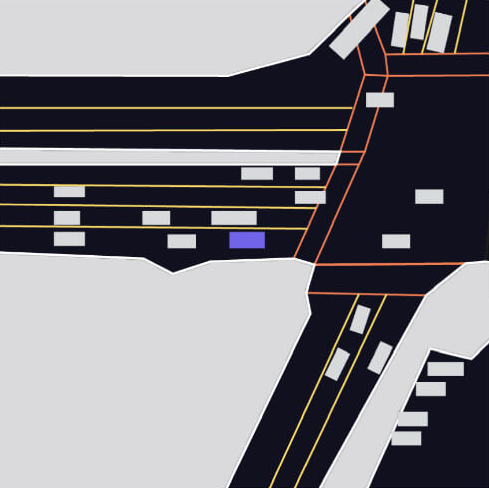
\includegraphics[width=0.47\linewidth]{pred_before.png} }}
    \qquad
    \subfloat[\centering Scena po predykcji]{{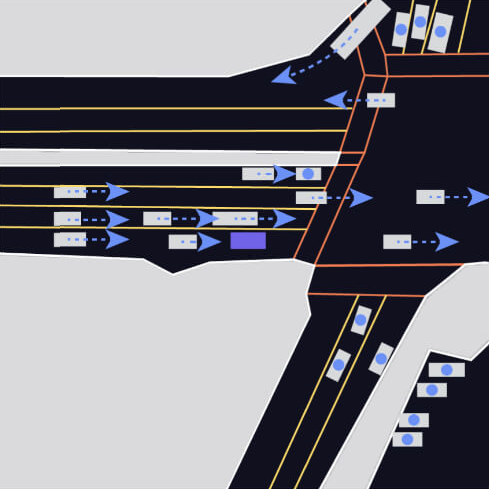
\includegraphics[width=0.47\linewidth]{pred_after.png} }}
    \caption{Wizualizacja problemu}
\end{figure}

\newpage

\section{Formalny opis problemu}

\noindent Problem poruszony w tej pracy polega na skonstruowaniu modelu predykcyjnego (funkcji $f$):
\begin{equation}
f(E_{t}, S_{t}, L_{t}) = ((V_{t}^{0}, P_{t}^{0}), (V_{t}^{1}, P_{t}^{1}), (V_{t}^{2}, P_{t}^{2}))
\end{equation}

\begin{conditions}
     E_{t}     &  Pozycje wejściowe agenta \texttt{EGO}, lista 11 pozycji \mbox{$[(x_{0},y_{0}), (x_{1},y_{1}), ... , (x_{10},y_{10})]$}, które zapisane są w odstępach 0.1 sekundy i dotyczą chwil \mbox{$[t, t-0.1, ... , t-1.0]$}\\
     S_{t}     &  Pozycje wejściowe agentów innych niż agent \texttt{EGO} (agenci są wybierani spośród otoczenia agenta \texttt{EGO}), jest to macierz w której każdy wiersz odpowiada wybranemu agentowi z otoczenia (innemu niż \texttt{EGO}), a każda kolumna odpowiada wybranej chwili w czasie. Komórka $S_{t}[i, j]$ zawiera współrzędne $(x, y)$ i-tego agenta  w chwili $t-j*0.1$ dla $j \in \{0, 1, ... , 10\}$.\\
     L_{t}     &  Lista wszystkich pasów ruchu i ich statusu przejezdności w chwili $t$. Każdy element to słownik z atrybutami \texttt{xyz\_left}, \texttt{xyz\_right}, \texttt{lights}. Atrybuty \texttt{xyz\_left}, \texttt{xyz\_right} zawierają listy współrzędnych węzłów interpolujących odpowiednio lewą i prawą krawędź pasa. Atrybut \texttt{lights} zawiera status przejezdności pasa. Wartość \texttt{'default'} (brak świateł) lub \texttt{'green'} oznacza, że pas jest przejezdny. Wartość \texttt{'red'} oznacza, że pas nie jest przejezdny.\\
     V_{t}^{k}     &  Dla $k \in \{0, 1, 2\}$ $V_{t}^{k}$ zawiera k-tą predykcję trajektorii ruchu agenta. Model nie musi przewidywać najbardziej prawdopodobnej trajektorii ruchu. Model może przewidzieć 3 trajektorie i każdej z nich przypisać prawdopodobieństwo z jaką dana trajektoria wystąpi. Lista $V_{t}^{k}$ zawiera 50 pozycji \mbox{$[(x_{0},y_{0}), (x_{1},y_{1}), ... , (x_{49},y_{49})]$}, które dotyczą chwil \mbox{$[t+0.1, t+0.2, ... , t+5.0]$}.\\
     P_{t}^{k}     &  Dla $k \in \{0, 1, 2\}$ $P_{t}^{k}$ zawiera przewidywane prawdopodobieństwo z jakim wystąpi ruch pojazdu po k-tej trajektorii (zostanie zrealizowana trasa zawarta w $V_{t}^{k}$). Zakłada się, że suma tych prawdopodobieństw wynosi $1$.
\end{conditions}

\section{Typ problemu}

Problem przewidywania pozycji wyjściowych agenta ruchu drogowego w chwili $t$, mając do dyspozycji pozycje wejściowe w chwili t, można rozważać jako problem uczenia nadzorowanego, gdzie na wejście modelu przekazuje się wszystkie dostępne informacje na temat sceny ruchu, a na wyjściu modelu otrzymuje się przewidywane trajektorie wybranego agenta ze sceny w ustalonym przedziale czasowym.

\section{Charakter problemu}

Problem przewidywania przyszłych pozycji obiektów uczestniczących w ruchu drogowym ma charakter praktyczny. Analizowany problem został zaczerpnięty z platformy \texttt{Kaggle}, gdzie firma \texttt{Lyft} ogłosiła konkurs na najlepszy system predykcyjny. Pula nagród wynosiła ponad 100 tys. zł. Firma \texttt{Lyft} ogłosiła konkurs w nadziei na pozyskanie inspiracji z interesujących rozwiązań, które mogłyby zostać zaimplementowane w autonomicznej flocie samochodów firmy \texttt{Lyft}. Zwiększenie skuteczności predykcji wiąże się bezpośrednio ze wzrostem bezpieczeństwa (pojazdy, mogą lepiej wnioskować na temat możliwych wariantów zachowań obiektów w otoczeniu), co w konsekwencji pozwoliłoby na zmniejszenie liczby ofiar oraz obrażeń ludzi w wypadkach z udziałem pojazdów autonomicznych (mowa tutaj o wszystkich markach samochodów, a nie tylko o samochodach organizatora konkursu).

\newpage

\section{Zbiór danych}

    Zbiór danych użyty w pracy to \texttt{Lyft Level5 Prediction Dataset} \cite{lyft2020}. Jest to największy udostępniony publicznie zbiór danych dotyczący przewidywania agentów ruchu ulicznego. Zbiór obejmuje zapisy trajektorii ruchu samochodów, rowerzystów, pieszych i innych agentów ruchu którzy znaleźli się w otoczeniu pojazdu zbierającego dane. Informacje te uzyskano poprzez przetwarzanie danych z lidaru, kamery i radaru za pośrednictwem systemów percepcji. Są to dane specjalnie przygotowane pod zadanie przewidywania ruchu. Zbiór danych obejmuje ponad tysiąc godzin zapisów z ruchu autonomicznych pojazdów firmy Lyft, ponad 25 tysięcy kilometrów zapisów z tras oraz ponad 15 tysięcy oznaczonych scen z otoczenia pojazdów (oznaczonych przez ludzi z wysoką dokładnością).

\vspace{1em}

W bibliotece \texttt{l5kit} używany jest format danych, który składa z tablic o strukturze podobnej do tablic biblioteki \texttt{numpy}. Jest podobny do zestawu plików \texttt{CSV} z wierszami i kolumnami, z tą różnicą, że są one przechowywane jako skompresowane pliki binarne zamiast tekstu. Tablice te mogą być bezpośrednio kopiowane z dysku do pamięci komputera, bez konieczności ich przetwarzania. Jest to wymagane, gdy mówimy o zbiorze który skompresowany zajmuje około 80GB i musi być bardzo szybko ładowany do pamięci RAM, aby w pełni wykorzystać potencjał szybkich operacji na GPU.

\vspace{1em}

Tablice przechowywane w formacie \texttt{zarr} pozwalają nam używać różnych typów danych w kolumnach w jednej tablicy, a reprezentacja bajtowa pozwala nam grupować próbki. Mając tak przygotowaną reprezentację odczytanie kilku przykładów ze zbioru ogranicza się do wczytania reprezentacji bitowej odpowiadających przykładów, nie trzeba wczytywać całego zbioru do pamięci i przetwarzać go. Biblioteka \texttt{zarr} obsługuje format danych \texttt{StructuredArrays}, który jest w pełni kompatybilny z tablicami biblioteki numpy.

\vspace{1em}

\section{Struktura zbioru danych}

Zbiór danych przechowywany jest w czterech uporządkowanych tablicach: \texttt{scenes}, \texttt{frames}, \texttt{agents} i \texttt{tl\_faces}.

\subsection{Tablica \texttt{scenes}}

\noindent
Struktura tablicy:

\begin{minted}{python}
SCENE_DTYPE = [
    ('frame_index_interval', np.int64, (2,)),  # para liczb typu int64
    ('host', '<U16'),  # ciąg znaków Unicode o długości <= 16
    ('start_time', np.int64),
    ('end_time', np.int64),
]
\end{minted}

\noindent
Unikalny identyfikator sceny to krotka (\texttt{host, start\_time, end\_time}).
Atrybut \texttt{host} to identyfikatur pojazdu, przez który zostały zebrane dane dotyczące danej sceny. Atrybuty \texttt{start\_time} oraz \texttt{end\_time} określają odpowiednio chwilę rozpoczęcia oraz chwilę zakończenia zapisywania danych dotyczących danej sceny. Scena składa się z wielu ramek (\texttt{frames}). Ramki to zbiory informacji na temat otoczenia w dyskretnych odstępach czasu. Scenę można porównać do filmu, który ma pewien okres trwania. Ramki można porównać do klatek filmu, czyli pojedynczych zdjęć zawierających informacje dotyczące danej chwili. Tablica \texttt{scenes} przechowuje odniesienia do odpowiednich ramek (\texttt{frames}) za pomocą indeksu początkowego i końcowego ramek. Wszystkie ramki pomiędzy tymi indeksami odpowiadają tej samej scenie.

\newpage

\subsection{Tablica \texttt{frames}}

\noindent
Struktura tablicy:

\begin{minted}{python}
FRAME_DTYPE = [
    ('timestamp', np.int64),
    ('agent_index_interval', np.int64, (2,)),
    ('traffic_light_faces_index_interval', np.int64, (2,)),
    ('ego_translation', np.float64, (3,)),
    ('ego_rotation', np.float64, (3, 3)),
]
\end{minted}

\noindent
Ramka (\texttt{frame}) zawiera wszystkie informacje, które były zaobserwowane w danej chwili, tzn:

\begin{itemize}
    \setlength{\itemsep}{1pt}
    \setlength{\parskip}{0.2em}
    \setlength{\parsep}{0.2em}
    \item \texttt{timestamp} - Znacznik czasu (czas uniksowy), opisywanej ramki.
    \item \texttt{agent\_index\_interval} - Przedział indeksów agentów, których agent \texttt{EGO} zaobserwował w otoczeniu.
    \item \texttt{traffic\_light\_faces\_index\_interval} - Przedział indeksów świateł drogowych, które agent \texttt{EGO} zaobserwował w otoczeniu.
    \item \texttt{ego\_translation} - Przemieszczenie agenta \texttt{EGO} (w metrach) względem punktu odniesienia $(0, 0, 0)$. Punkt ten ma współrzędne geograficzne \mbox{(37°25'45.6$"$N, 122°09'15.7$"$W, 0 m n.p.m.)}, znajduje się w Palo Alto (Kalifornia).
    \item \texttt{ego\_rotation} - Macierz $(3\times3)$ rotacji agenta \texttt{EGO} względem wektora $(1, 0, 0)$ z punktem przyłożenia równym $(0, 0, 0)$.
\end{itemize}

\noindent
Właściwości zarówno agentów, jak i sygnalizacji świetlnej są przechowywane w tablicach \texttt{agents} i \texttt{tl\_faces}. Ramka zawiera tylko odniesienia (przedziały indeksów) do tych obiektów podane przez indeks początkowy i końcowy w atrybutach \texttt{agent\_index\_interval} i \texttt{traffic\_light\_faces\_index\_interval}.

\subsection{Tablica \texttt{agents}}

\noindent
Struktura tablicy:

\begin{minted}{python}
AGENT_DTYPE = [
    ('centroid', np.float64, (2,)),
    ('extent', np.float32, (3,)),
    ('yaw', np.float32),
    ('velocity', np.float32, (2,)),
    ('track_id', np.uint64),
    ('label_probabilities', np.float32, (len(PERCEPTION_LABELS),)),
]
\end{minted}

\noindent
Wiersz tablicy \texttt{agents} zawiera informacje na temat pewnego agenta (agenta z otoczenia agenta \texttt{EGO}) z ramki, które były zaobserwowane w danej chwili (chwili zapisanej w atrybucie \texttt{timestamp} tablicy \texttt{frames}, z której odnosimy się do agenta tablicy \texttt{agents}). Szczegółowe informacje na temat agentów zawarte w tablicy \texttt{agents}:

\begin{itemize}
    \setlength{\itemsep}{1pt}
    \setlength{\parskip}{0.2em}
    \setlength{\parsep}{0.2em}
    \item \texttt{centroid} - Przemieszczenie agenta (w metrach) względem punktu odniesienia $(0, 0)$. Punkt ten ma współrzędne geograficzne \mbox{(37°25'45.6$"$N, 122°09'15.7$"$W)}, znajduje się w Palo Alto (Kalifornia).
    \item \texttt{extent} - Wymiary agenta $(x,y,z)$ (szerokość, długość, wysokość)
    \item \texttt{yaw} - Odchylenie agenta względem wektora $(1, 0)$ z punktem przyłożenia równym $(0, 0)$.
    \item \texttt{velocity} - Szybkość ruchu agenta względem osi $x$ oraz $y$.
    \item \texttt{track\_id} - Identyfikator agenta, który pozwala wyszukiwać tego samego agenta w wielu ramkach.
    \item \texttt{label\_probabilities} - Wektor prawdopodobieństw przynależności do klas z listy \texttt{PERCEPTION\_LABELS}
\end{itemize}

\begin{minted}{python}
PERCEPTION_LABELS = [
    'PERCEPTION_LABEL_NOT_SET',
    'PERCEPTION_LABEL_UNKNOWN',
    'PERCEPTION_LABEL_DONTCARE',
    'PERCEPTION_LABEL_CAR',
    'PERCEPTION_LABEL_VAN',
    'PERCEPTION_LABEL_TRAM',
    'PERCEPTION_LABEL_BUS',
    'PERCEPTION_LABEL_TRUCK',
    'PERCEPTION_LABEL_EMERGENCY_VEHICLE',
    'PERCEPTION_LABEL_OTHER_VEHICLE',
    'PERCEPTION_LABEL_BICYCLE',
    'PERCEPTION_LABEL_MOTORCYCLE',
    'PERCEPTION_LABEL_CYCLIST',
    'PERCEPTION_LABEL_MOTORCYCLIST',
    'PERCEPTION_LABEL_PEDESTRIAN',
    'PERCEPTION_LABEL_ANIMAL',
    'AVRESEARCH_LABEL_DONTCARE',
]
\end{minted}

\subsection{Tablica \texttt{tl\_faces} (sygnalizacji świetlnej)}

\noindent
Struktura tablicy:

\begin{minted}{python}
TL_FACE_DTYPE = [
    ("face_id", "<U16"),
    ("traffic_light_id", "<U16"),
    ("traffic_light_face_status", np.float32, (len(TL_FACE_LABELS,))),
]

TL_FACE_LABELS = [
    'ACTIVE',
    'INACTIVE',
    'UNKNOWN',
]
\end{minted}

\noindent
Wiersz tablicy \texttt{tl\_faces} zawiera informacje o elemencie sygnalizacji świetlnej:

\begin{itemize}
    \setlength{\itemsep}{1pt}
    \setlength{\parskip}{0.2em}
    \setlength{\parsep}{0.2em}
    \item \texttt{face\_id} - Identyfikator pojedynczej żarówki na elemencie sygnalizacji świetlnej.
    \item \texttt{traffic\_light\_id} - Identyfikator zbioru żarówek na elemencie sygnalizacji świetlnej (tutaj poprzez \texttt{traffic\_light} rozumie się element sygnalizacji świetlnej jako całość, może posiadać kilka żarówek)
    \item \texttt{traffic\_light\_face\_status} - Status zbioru żarówek (mówi o tym czy sygnalizacja świetlna jest aktywna lub wyłączona z użytku)
\end{itemize}

\noindent
Trzeba zaznaczyć, że elementy tablicy \texttt{tl\_faces} nie zawierają informacji o tym czy dana żarówka się świeci, czy nie. Elementy mówią nam czy dana żarówka jest aktywna (czyli czy normalnie funkcjonuje). Dynamiczną informację o tym czy żarówka się świeci czy nie możemy uzyskać z niżej opisanego pliku \texttt{semantic\_map.pb}, który mówi między innymi kiedy żarówka się świeci (zawiera informację o cyklu działania)
\newpage

\subsection{Mapa i obiekty świata}

\noindent
Bardzo istotnym elementem zbioru jest opis świata zawarty w pliku \texttt{semantic\_map.pb} w formacie \texttt{Protocol Buffers}. Plik ten zawiera między innymi obiekty następujących klas (wymienione tylko najważniejsze):
    \begin{itemize}
    \setlength{\itemsep}{1pt}
    \setlength{\parskip}{0.2em}
    \setlength{\parsep}{0.2em}
    \item \texttt{GEOLOCATION} - Klasa która zawiera informację o lokalizacji obiektu na mapie, obiekty tej klasy są zawarte we wszystkich niżej wymienionych klasach.
    \item \texttt{JUNCTION} - Klasa zawierająca opis skrzyżowania, zawiera informację o tym jakie drogi są z nim połączone oraz jakie elementy sygnalizacji świetnej są w nim zawarte.
    \item \texttt{ROADNETWORKSEGMENT} - Klasa zawierająca opis kawałka drogi, czyli wszyskich pasów ruchu które są w tym kawałku drogi zawarte.
    \item \texttt{ROADNETWORKSEGMENT\_TRAVELDIRECTION} - Klasa opisująca w którą stronę odbywa się ruch na kawałku drogi oraz panujące na nim zasady ruchu.
    \item \texttt{LANESEQUENCE} - Klasa opisująca ciąg pasów ruchu wykorzystywany przez klasę \texttt{ROADNETWORKSEGMENT}.
    \item \texttt{LANE} - Klasa opisująca pojedynczy pas ruchu.
    \item \texttt{LANE\_BOUNDARY} - Klasa opisująca granice pasu ruchu.
    \item \texttt{TRAFFICCONTROLELEMENT\_PEDESTRIANCROSSWALK} - Klasa opisująca przejście dla pieszych.
    \item \texttt{TRAFFICCONTROLELEMENT\_TRAFFICLIGHTFACESTATE} - Klasa opisująca stan pojedynczej żarówki, na elemencie sygnalizacji świetlnej (zawiera informację o tym jaki jest cykl włączania i wyłączania żarówki)
    \item \texttt{TRAFFICCONTROLELEMENT\_TRAFFICLIGHT} - Klasa opisująca element sygnalizacji świetlnej (zbiór żarówek)
\end{itemize}

\section{Interfejsy zbioru}
\subsection{\texttt{ChunkedDataset}}

Jest to pierwszy interfejs między surowymi danymi na dysku, a skryptem języka \texttt{Python}. Ten interfejs jest bardzo prosty i zwraca cztery tablice (\texttt{scenes}, \texttt{frames}, \texttt{agents} i \texttt{tl\_faces}) wczytane wprost z dysku. Gdy w skrypcie odnosimy się do jednej z tych tablic, biblioteka \texttt{zarr} identyfikuje fragment tablicy do załadowania, fragment ten jest dekompresowany w locie, a na końcu zwracana jest kopia fragmentu w formacie tablicy \texttt{numpy}.

\vspace{1em}

Praca z surowym zbiorem danych w formacie \texttt{zarr} (np. poprzez interfejs \texttt{ChunkedDataset}), nie jest zalecana. Bardzo łatwo o pomyłkę, która w przypadku trenowania głębokich sieci neuronowych przy tak ogromnym zbiorze, może być niemożliwa do wychwycenia. Aby uniknąć pomyłek w implementacji procesowania zbioru biblioteka \texttt{l5kit} zapewnia dwie struktury, które tworzą dodatkową warstwę abstrakcji nad surowym zbiorem danych w formacie \texttt{zarr}. Te dwie klasy pozwalają na rasteryzację i uzyskanie informacji o pozycjach wejściowych i wyjściowych agentów w wielu scenach. Opisane poniżej klasy dziedziczą po klasie \texttt{Pytorch Dataset} i są z nią ściśle powiązane. Umożliwia to efektywne wykorzystanie obiektu \texttt{Pytorch Dataloader} do wielowątkowej rasteryzacji scen. Poniższe klasy zakładają, że świat jest rasteryzowany w reprezentacji \texttt{BEV} (widok z lotu ptaka), co jest typowym wyborem dla podejść opartych o głębokie sieci neuronowe, w szczególności sieci typu \texttt{CNN} (konwolucyjne sieci neuronowe).

\newpage

\subsection{\texttt{EgoDataset}}

Klasa \texttt{EgoDataset} pozwala na iterowanie po elementach zbioru w kolejności, która skupia się na pojeździe zbierającym dane (agenci \texttt{EGO} w przypadku zbioru \texttt{EgoDataset} są tylko i wyłącznie pojazdami firmy \texttt{Lyft}). Elementy zbioru są posortowane kluczem (indeks sceny, indeks ramki, indeks agenta). Oznacza to, że iterując po kolejnych elementach zbioru otrzymamy kolejne ramki z trasą samochodu zbierającego dane (agentem \texttt{EGO} nie będzie np. pieszy lub rowerzysta).

\begin{center}
\begin{tabular}{ | m{4cm} | m{12cm}| } 
\hline
\texttt{image} & Raster \texttt{BEV} jako wielokanałowy obraz\\
\hline
\texttt{target\_positions} & Wyjściowe współrzędne agenta \texttt{EGO} (w systemie odniesienia agentów w metrach).\\
\hline
\texttt{target\_yaws} & Wyjściowe kąty odchylenia agenta \texttt{EGO} (w radianach).\\
\hline
\texttt{target\_availabilities} & Wektor zawierający wartość 1, gdy pozycja agenta \texttt{EGO} ma znaczenie lub 0, gdy pozycja agenta \texttt{EGO} nie ma znaczenia. Na końcu lub na początku sceny mogą wystąpić nieprawidłowe pozycje, wektor \texttt{target\_availabilities}, mówi kiedy je zignorować. Wektor dotyczy pozycji wyjściowych\\
\hline
\texttt{history\_positions} & To samo, co \texttt{target\_positions}, ale dotyczy pozycji wejściowych.\\
\hline
\texttt{history\_yaws} & To samo co \texttt{target\_yaws}, ale dotyczy pozycji wejściowych.\\
\hline
\texttt{history\_availabilities} & To samo co \texttt{target\_availabilities}, ale dotyczy pozycji wejściowych.\\
\hline
\texttt{raster\_from\_world} & Macierz $(3\times3)$ przekształcająca współrzędne z systemu odniesienia świata do systemu odniesienia obrazu.\\
\hline
\texttt{raster\_from\_agent} & Macierz $(3\times3)$ przekształcająca współrzędne z systemu odniesienia agenta \texttt{EGO} do systemu odniesienia obrazu.\\
\hline
\texttt{agent\_from\_world} & Macierz $(3\times3)$ przekształcająca współrzędne z systemu odniesienia świata do systemu odniesienia agenta \texttt{EGO}.\\
\hline
\texttt{world\_from\_agent} & Macierz $(3\times3)$ przekształcająca współrzędne z systemu odniesienia agenta \texttt{EGO} do systemu odniesienia świata.\\
\hline
\texttt{track\_id} & Unikalny identyfikator sceny.\\
\hline
\texttt{timestamp} & Czas uniksowy chwili bieżącej ramki.\\
\hline
\texttt{centroid} & Środek agenta \texttt{EGO} w bieżącej ramce w układzie odniesienia świata (jednostka metry).\\
\hline
\texttt{yaw} & Kąt odchylenia agenta \texttt{EGO} w bieżącej klatce w układzie odniesienia świata (jednostka radiany).\\
\hline
\texttt{extent} & Wymiary agenta \texttt{EGO} (XYZ: szerokość, długość, wysokość) w układzie odniesienia świata (jednostka metry).\\
\hline
\end{tabular}
\end{center}

\subsection{\texttt{AgentDataset}}

\texttt{AgentDataset} wykonuje iteracje po agentach (tzn. każdej dynamicznej jednostce na scenie) zamiast kolejno po ramkach zapisanych przez pojazd zbierający dane. Zwrócony słownik jest dokładnie taki sam jak w przypadku klasy \texttt{EgoDataset}. Te dwie klasy są prawie takie same, istnieje jednak jedna fundamentalna różnica: \texttt{AgentDataset} wykorzystuje maskę agentów, która określa, które obiekty powinny być uwzględnione w danej scenie. Jest to używane podczas wykluczania niewiarygodnych agentów podczas procesu trenowania i testowania modeli (np. agentów poniżej pewnego progu prawdopodobieństwa klasy) lub aby wybrać podzbiór agentów (np. podczas ewaluacji modelu, aby uniknąć przypisywania dużej wartości funkcji kosztu poprawnym predykcjom, które zostały omyłkowo niepoprawnie zaznaczone w zbiorze). Jeśli maska nie zostanie przekazana jako argument do obiektu klasy \texttt{AgentDataset}, nowa zostanie obliczona na podstawie wartości parametru \texttt{filter\_agents\_threshold}.

\newpage

\subsection{Podział zbioru danych}

\noindent
Zbiór danych został podzielony na 3 rozłączne podzbiory:

\begin{itemize}
    \setlength{\itemsep}{1pt}
    \setlength{\parskip}{0.2em}
    \setlength{\parsep}{0.2em}
    \item \textbf{treningowy} - Zbiór składający się z 198 mln ramek, skompresowany zajmuje 72 GB. Zbiór ten został użyty w procesie trenowania modeli opisanych w tej pracy. Zbiór jest tak duży, że nie udało się wytrenować modeli na wszystkich jego elementach. W procesie trenowania wszystkich modeli użyto zaledwie ok. 30\% elementów zbioru (proces trenowania trwał około 3 tygodnie).
    \item \textbf{walidacyjny} - Zbiór składający się z 5 tys. ramek. Używany do szybkiego monitorowania procesu trenowania (jest mały ze względu na oszczędność czasu predykcji).
    \item \textbf{testowy} - Zbiór składający się ze 100 tys. ramek, używany do ostatecznej oceny skuteczności predykcji modeli.
\end{itemize}

W literaturze naukowej bardzo często spotyka się podział zbioru na treningowy, walidacyjny i testowy w proporcjach 0.6, 0.2, 0.2. W tej pracy dysproporcja pomiędzy wielkościami zbiorów jest bardzo duża 198 mln, 5 tys. , 100 tys. , jest to w pełni zamierzone działanie, które ma na celu jak najefektywniejsze wykorzystanie zbioru. Taki podział sprawia, że modele są trenowane na bardzo różnorodnym zbiorze treningowym. Zbiór walidacyjny jest mały, dzięki czemu można szybko i często monitorować skuteczność modelu (z wariancją na akceptowalnym poziomie). Zbiór testowy jest na tyle duży, aby zapewnić minimalny wpływ losowości na wynik uśrednionej funkcji kosztu (zapewnić małą wariancję).